\chapter{Sequence Modeling: Recurrent and Recursive Networks}

Recurrent Neural Networks are a type of Neural Network architecture that works with sequential data. This is data structured in a sequence where the order holds significance and carries information. Examples: speech and audio data, time series data, textual data, ... 

\noindent Previously we have seen Feedforward Neural Networks and Convolutional Neural Networks architectures. These architectures have what is called a one to one relationships as they both have a fixed size input, a set of hidden layers and finally a single output (or output set). Instead when working with sequential data, we can have:

\begin{itemize}
    \item Many to One Relationships. These are used in sequence classification tasks (e.g. Sentiment classification) which imply having sequential inputs and a single output or output set. 
    \item One to Many Relationships. These architectures are used in sequence generations tasks (e.g. Image Captioning) which is composed of a single input and a sequential output.
    \item Many to many Relationships. These are used in sequence transductions tasks (e.g. Machine translation) which consists of a sequential input and sequential output. In the specific case where we have the same length for both the input and the output we are in an IO-transduction (e.g. Phoneme recognition system).
\end{itemize}

\begin{figure}[h]
    \centering
    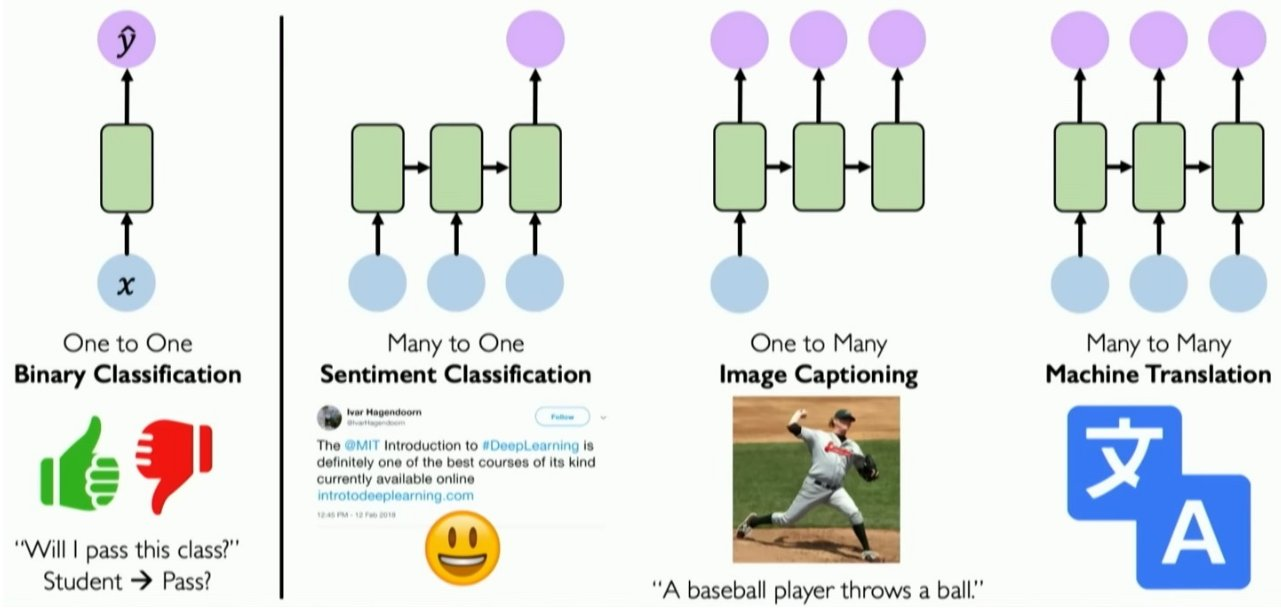
\includegraphics[width=15cm]{Images/sequence-to-sequence.jpg}
    \caption{Sequence to sequence }
    \label{fig:sequence-to-sequence}
\end{figure}

\newpage
\section{Sequential Transduction}

A sequential transduction $T$ refers to the transformation of an input sequence $X = x^{(1)}, ..., x^{(n)}$ into the corresponding output sequence $Y=y^{(1)}, ..., y^{(m)}$ where $n$ and $m$ are the length of the input and output sequences respectively.

\subsection{Memory}

A sequential transduction $T$ has finite memory $k \in N$ if $ \forall ~ x \in X$ and $\forall ~ t, T(x^{(t)})$ only depends on the sequence $ \left ( x^{(t)}, x^{(t-1)}, ..., x^{(t-k)}  \right ) $. Basically this means that its transformation process only requires a bounded and limited amount of information from the input sequence's past elements to produce the output sequence.

\begin{figure}[h]
    \centering
    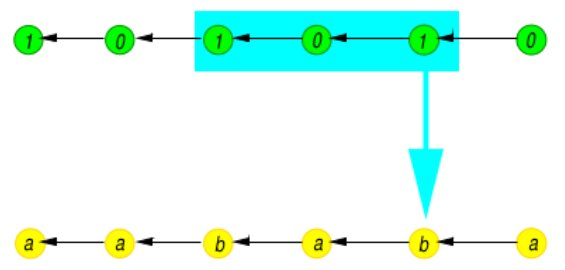
\includegraphics[width=6cm]{Images/transduction-memory.jpg}
    \caption{Transduction Memory}
    \label{fig:transduction-memory}
\end{figure}

\noindent A sequential transduction $T$ is algebraic if it has 0 memory ($k=0$) meaning that its transformation process is solely determined by the input element at the current position $x^{(t)}$ and does not rely on any previous elements in the sequence. An algebraic transduction is memory-less.

\subsection{Causality}

A sequential transduction $T$ is casual if the output at time $t$ does not depend on future inputs (at time $t+1$, $t+2$, ...). In sequential transductions, causality is respected, meaning that the transformation of an element in the output sequence depends only on the elements that have already appeared in the input sequence.

\begin{figure}[h]
    \centering
    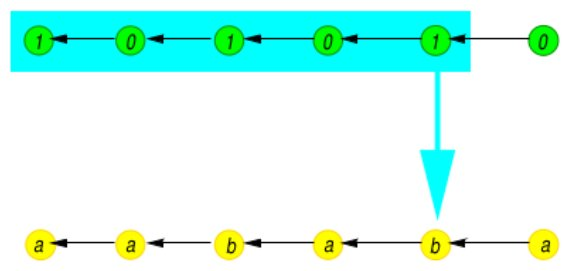
\includegraphics[width=6cm]{Images/causality.jpg}
    \caption{Causality}
    \label{fig:causality}
\end{figure}

\subsection{Stationary}

A sequential transduction $T$ is stationary if the transformation it applies to the input sequence $T(x^{(t)})$ is independent of the position within the sequence. In other words, we will get the same outcome regardless of the value of $t$.

\newpage
\section{Recurrent Neural Network Architecture}

Recurrent Neural Networks are based on the idea of employing recurrent units that maintain hidden states. These states capture information from the current input and the previous hidden state, allowing the network to learn and remember patterns across time steps. The basic Recurrent Neural Network unit takes an input vector $x^{(t)}$ at time step $t$ and a hidden state vector $h^{(t-1)}$ from the previous time step in order to compute the new hidden state $h^{(t)}$:

$$ h^{(t)} = \sigma \left( U x^{(t)} +  W h^{(t-1)} \right ) $$

\noindent where U and W are the weight matrices for the current and previous state. The network returns an output o at a given time-step t:

$$ o^{(t)} = \sigma \left( V h^{(t)} \right) $$

\noindent For every time step the Recurrent Neural Network has only a single hidden layer which maintains a hidden $ h^{(t)}$ at each time step $t$, and this is updated sequentially as the Recurrent Neural Network processes the input sequence.

\noindent To process a sequence of inputs $x^{(t)}$ we apply the basic Recurrent Neural Network unit at each time step t. We can unroll this loop-like diagram in order to represent the Recurrent Neural Network as a computational graph unrolled across time.

\begin{figure}[h]
    \centering
    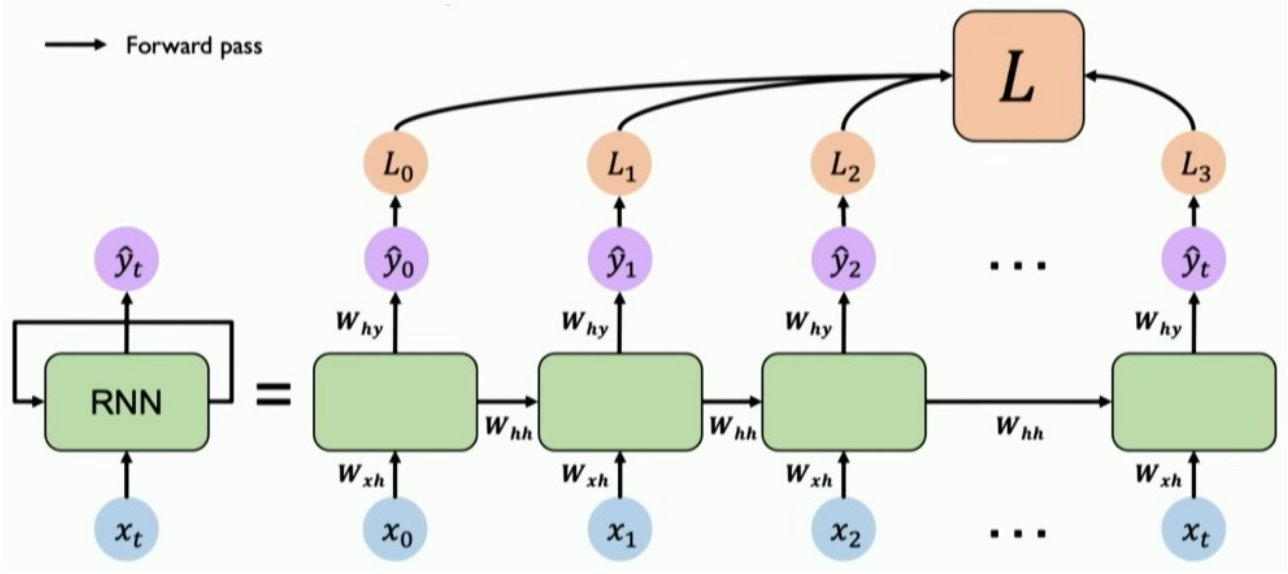
\includegraphics[width=15cm]{Images/rnn.jpg}
    \caption{Recurrent Neural Network Unrolled}
    \label{fig:rnn}
\end{figure}

\newpage
\noindent We can also describe the hidden representation in a Recurrent Neural Network as:

$$ q^{-1} h^{(t)} = h^{(t-1)} $$

Where $q$ is a unitary time delay operator, which means it shifts the hidden state representation $h^{(t)}$ from the current time step $t$ to the next time step $t + 1$. As you can guess $q^{-1}$ does the inverse operation of q. It shifts the hidden state representation $h^{(t)}$ from the current time step $t$ to the previous time step $t - 1$.

\begin{figure}[h]
    \centering
    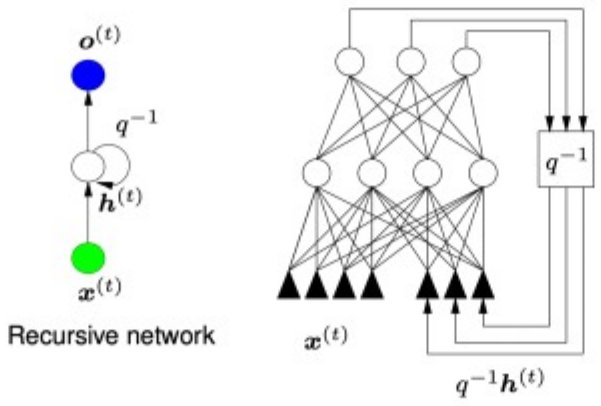
\includegraphics[width=9cm]{Images/rnn-time-delay.jpg}
    \caption{Recurrent Neural Network with time delay representation}
    \label{fig:rnn-time-delay}
\end{figure}

\section{Algorithm}

The overall Recurrent Neural Network algorithm works as follows:

\noindent At the beginning of the sequence processing we initialize the hidden state $h^{(0)}$ to small random values. We will also initialize in the same way the training matrices $U$, $W$ and $V$, and biases $b$ and $c$. We will also set the hyper-parameters which include the learning rate, number of hidden units, activation functions used in the hidden layers, the batch size, ... Now for every time step $ t = 1, ..., T$ we compute the linear transformation of the current input $x^{(t)}$ using the input-to-hidden weights matrix $U$:

$$ U x^{(t)}$$

\noindent This represents the transformed input information at time step $t$. It is often referred to as the pre-activation because it determines how much influence the current input $x^{(t)}$ should have on the new hidden state $h^{(t)}$. Each row of $U$ corresponds to a hidden unit in the Recurrent Neural Network, and each column corresponds to an element in the input at step t $x^{(t)}$. The weights of the matrix control how much each element in the input will contribute.

\noindent Now we compute the linear transformation of the previous hidden state $h^{(t - 1)}$ using the hidden-to-hidden weight matrix $W$.

$$ W h^{(t-1)} $$

\noindent The $W$ matrix determines how information from the previous time step is carried over to the current time step. Each row of $W$ corresponds to a hidden unit, and each column corresponds to a hidden unit from the previous time step.
We can apply an activation function to the combination of both results adding a bias term b to get the hidden state of the actual time step t.

$$ h^{(t)} = \sigma \left( U x^{(t)} + W h^{(t-1)} + b \right) $$

\noindent Finally, compute the output $o^{(t)}$ of the current time-step using the hidden state $h^{(t)}$ and the matrix $V$.

$$ o^{(t)} = \sigma \left(V h^{(t)} + c \right) $$

where the matrix $V$ defines how the information of the hidden state is used to generate the output at each time step. This will be the case if our Recurrent Neural Network is designed for sequence-to-sequence or vector to sequence tasks as an output $o^{(t)}$ will be generated for every time-step in the sequence. The final output is the sequence of all the individual outputs $o^{(t)}$, generated at each time step t:

$$ o = \left[ o^{(1)},  o^{(2)}, ...,  o^{(T)} \right]  $$

\noindent If instead we have a sequence to single output architecture we will get the result $o$ as:

$$ o^{(T)} = \sigma \left(V h^{(T)} + c \right) $$

\noindent By comparing the generated output sequence to the target sequence we can calculate the loss L. 

$$L = - \sum_{t} log (p_{model}) = - \sum_{t} log \left( p \left( y^{(t)} | x^{(1)}, ..., x^{(t)} \right) \right)$$

\noindent which we can use to update the model parameters, by computing the gradients of the loss with respect to them using either Back-Propagation Through Time (BPTT) or Real-Time Recurrent Learning algorithms. This will allow us to update the model parameters using a gradient descent algorithm (e.g. SGD, Adam, etc.) with a learning rate $\eta$. This can be repeated by a number of epochs N in order to improve the network results minimizing the loss.


\section{BPTT vs RTRL}

Backpropagation Through Time and Real-Time Recurrent Learning are two different algorithms used in training Recurrent Neural Networks. They both address the challenge of training networks with temporal dependencies, but they do so in distinct ways.

\subsection{Back-Propagation Through Time}

Back-Propagation Through Time is typically used in a batch learning setting. it involves processing the entire sequence and accumulating the gradients over the entire sequence before performing a weight update. We will start the backward pass from the last time step $t = T$ and work backwards to $t = 1$. So given the loss at each time step $L(t)$ we will start by computing the gradient of the loss with respect to the output matrix $V$.

$$ \frac{\partial L^{(T)}}{\partial V } = \frac{\partial L^{(T)}}{\partial o^{(T)} } \frac{\partial o^{(T)}}{\partial V } $$


\noindent Then we can compute the gradient of the loss with respect to the hidden to hidden state matrix $W$ and the input to hidden state matrix $U$.

$$ \frac{\partial L^{(T)}}{\partial W } =  \frac{\partial L^{(T)}}{\partial o^{(T)} } \frac{\partial o^{(T)}}{\partial W } ~~~~~ \frac{\partial L^{(T)}}{\partial U } =  \frac{\partial L^{(T)}}{\partial o^{(T)} } \frac{\partial o^{(T)}}{\partial U }
$$

\newpage
\noindent In order to get these two values we will need to apply the chain rule:

$$ \frac{\partial o^{(T)}}{\partial W} = \sum_{t'=1}^{T} \frac{\partial o^{(T)}}{\partial h^{(T)}} \frac{\partial h^{(T)}}{\partial h^{(t')}} \frac{\partial h^{(t')}}{\partial W} ~~~~~~~ \frac{\partial o^{(T)}}{\partial U} = \sum_{t'=1}^{T} \frac{\partial o^{(T)}}{\partial h^{(T)}} \frac{\partial h^{(T)}}{\partial h^{(t')}} \frac{\partial h^{(t')}}{\partial U} $$

\noindent Where

$$ \frac{\partial h^{(t)}}{\partial h^{(t')}} = \prod_{j=t'+1}^{t} \frac{\partial h^{(j)}}{\partial h^{(j-1)}}$$

\begin{figure}[h]
\centering     %%% not \center
\subfigure[Backpropagation of gradient W]{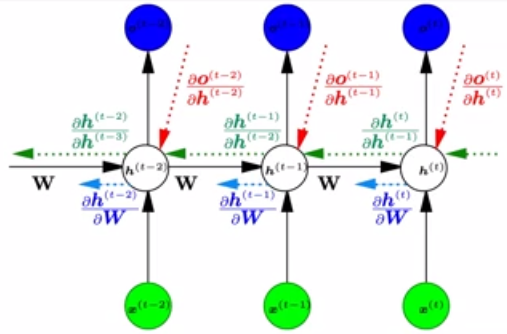
\includegraphics[width=7cm]{Images/bptt-w-matrix.png}}
\subfigure[Backpropagation of gradient U]{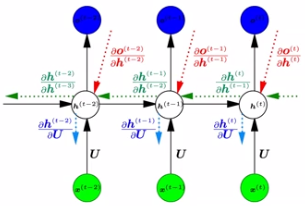
\includegraphics[width=7cm]{Images/bptt-u-matrix.png}}
\end{figure}


\noindent Notice that because Recurrent Neural Networks computations at each time step are dependent on the computations from the previous time step, we will need to propagate the gradients backwards in time, starting from the last time step.

\noindent This is then repeated for every time step. At the end of this process, you will have computed the gradients of the loss with respect to the three weight matrices for each time step $t$. Summing the values for each time step will give us the total gradient values.

$$ \frac{\partial L}{\partial V } = \sum_{t=1}^{T} \frac{\partial L^{(t)}}{\partial V } ~~~~~ \frac{\partial L}{\partial W } = \sum_{t=1}^{T} \frac{\partial L^{(t)}}{\partial W }  ~~~~~ \frac{\partial L}{\partial U } = \sum_{t=1}^{T} \frac{\partial L^{(t)}}{\partial U } $$

\noindent We can use that to update the weight matrices $U$, $V$ and $W$ using an optimization algorithm based on gradient descent.

$$ U \leftarrow U - \eta \frac{\partial L}{\partial U}  ~~~~~ V \leftarrow V - \eta \frac{\partial L}{\partial V} ~~~~~ W \leftarrow W - \eta \frac{\partial L}{\partial W}$$

\newpage
\subsection{Real Time Recurrent Learning}
 
Instead, Real Time Recurrent Learning is designed for online learning, as it updates the gradient at each forward propagation step. This makes this algorithm suitable for real-time applications where updates need to be made continuously every time you receive a new input. Real Time Recurrent Learning directly computes the gradients of the loss with respect to the weights using the exact equations for Recurrent Neural Networks, without unrolling the network.

 Therefore, instead of waiting to compute the whole Loss for the entire sequence and then calculate the gradients by backpropagation, we will be able to compute the gradient in the forward phase. Given a time step $t$ we can consider computing the gradient up to that time step by back-propagating from that time step backwards. Starting at $t=1$ we will be able to compute the gradient at that time step and update the weights. Then we will move forward, and do the same for every time step by remembering that the gradient of the loss up to time $t$ can be computed just by adding the gradient at time $t$ to the previous gradient up to time $t-1$. By doing this from $t=1$ to $t=T$ we will end up computing the same gradient as when performing the Back-Propagation Through Time algorithm.

$$ \frac{\partial L|_t}{\partial V} =  \sum_{t=1}^{t} \frac{\partial L^{(t)}}{\partial o^{(t)} } \frac{\partial o^{(t)}}{\partial V  } = \frac{\partial L|_{t-1}}{\partial V} + \frac{\partial L^{(t)}}{\partial o^{(t)} } \frac{\partial o^{(t)}}{\partial V  }  $$

\noindent In the same way:

$$ \frac{\partial L|_t}{\partial U} =  \sum_{t=1}^{t} \frac{\partial L^{(t)}}{\partial o^{(t)} } \frac{\partial o^{(t)}}{\partial U  } = \frac{\partial L|_{t-1}}{\partial U} + \frac{\partial L^{(t)}}{\partial o^{(t)} } \frac{\partial o^{(t)}}{\partial U  } ~~~~~  \frac{\partial L|_t}{\partial W} =  \sum_{t=1}^{t} \frac{\partial L^{(t)}}{\partial o^{(t)} } \frac{\partial o^{(t)}}{\partial W  } = \frac{\partial L|_{t-1}}{\partial W} + \frac{\partial L^{(t)}}{\partial o^{(t)} } \frac{\partial o^{(t)}}{\partial W  }  $$

\noindent The downside of Real Time Recurrent Learning is that usually the amount of memory and time to compute it is larger than while performing Back-Propagation Through Time. This is why unless you are performing online learning this algorithm is not used so much. 

\begin{table}[h!]
\centering
\begin{tabular}{ p{6cm} p{3cm} p{3cm} } 
\hline\hline
\multirow{2}{*}{Algorithm} & \multicolumn{2}{c}{Complexity}\\ \cline{2-3}\\ & Space & Time \\ \hline

Back-Propagation Through Time & $O(NT)$ & $O(N^{2}T)$ \\ 
Real Time Recurrent Learning & $O(N^{3})$ & $ O(N^{4})$ \\
\hline
\end{tabular}
\end{table}

\noindent As you can see,  Real Time Recurrent Learning will only be more efficient than Back-Propagation Through Time when the number of time steps $T$ is very big. Specifically when $T > N^{2}$ where $N$ is the number of units.

\newpage
\section{Additional Architectural Features for Recurrent Neural Networks}

We can add features to the Vanilla Recurrent Neural Network architecture that make the network behave differently. Let's review some of them:

\subsection{Short-cut Connections}

Short-cut Connections. Shortcut connections, are used to skip some of the connections between the input and the hidden layers, effectively bypassing some of the intermediate layers.

\begin{figure}[h]
    \centering
    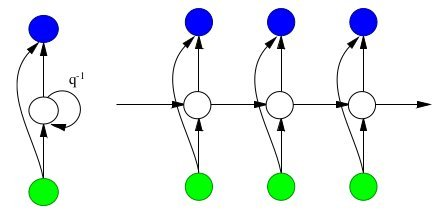
\includegraphics[width=8cm]{Images/short-cut-RNN.jpg}
    \caption{Shortcut in A Recurrent Neural Network}
    \label{fig:shortcut}
\end{figure}

\noindent The output $o^{(t)}$ then will be:

$$ o^{(t)} = \sigma \left(V^{h} h^{(t)} + V^{x} x^{(t)} + c \right) $$

Now both the hidden state $h^{(t)}$ and the input $x^{(t)}$ contribute to the output $o^{(t)}$ (via $V^{h}$ and $V^{x}$ respectively). This means that the network takes both the historical context represented by the hidden state and the current input into account when making predictions.

\subsection{Higher Order States}

Higher order states refer to hidden states that capture dependencies beyond just the immediately preceding time step. In a standard Recurrent Neural Network, the hidden state at a given time step is typically based on the input at that time step and the hidden state at the previous time step. However, higher-order states go beyond this one-step dependency and capture information from further back in the sequence.

\begin{figure}[h]
    \centering
    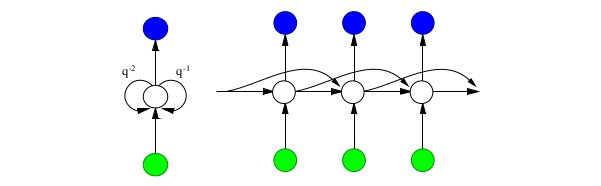
\includegraphics[width=12cm]{Images/higher-order-RNN.jpg}
    \caption{2nd Order State}
    \label{fig:higher-order}
\end{figure}

\noindent The hidden state $h^{(t)}$ then will be:

$$ h^{(t)} = \sigma \left( U x^{(t)} + W^{(1)} h^{(t-1)} + W^{(2)} h^{(t-2)} + b \right) $$

\subsection{Feedback from Output}

Feedback from the output relates to how the network's own predictions at a previous time step can influence the predictions it makes at the current or subsequent time steps. This feedback loop can have a significant impact on the network's behavior and is related to the concept of teacher forcing in training Recurrent Neural Networks. 

\begin{figure}[h]
    \centering
    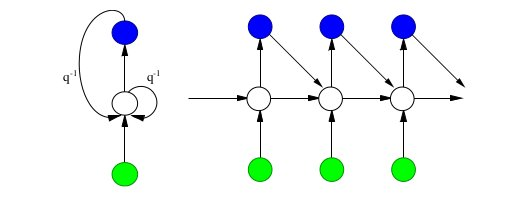
\includegraphics[width=10cm]{Images/output-feedback.jpg}
    \caption{Output Feedback in a RNN architecture}
    \label{fig:output-feedback}
\end{figure}

\noindent This modifies the hidden state in the following way:

$$ h^{(t)} = \sigma \left( U x^{(t)} + W h^{(t-1)} + Z o^{(t - 1)} + b \right) $$

\noindent Feedback from the output can be a useful technique for capturing dependencies and maintaining context.

\subsection{Teacher Forcing}

Teacher forcing is very similar to feedback from the output feature but instead of providing the last step prediction the hidden state takes as input the last step true target. This reduces the accumulation of errors, allowing the network to learn from its mistakes quickly. However, this can lead to exposure bias, where the model struggles to generate sequences independently during inference because it hasn't learned to cope with its own errors.

\begin{figure}[h]
    \centering
    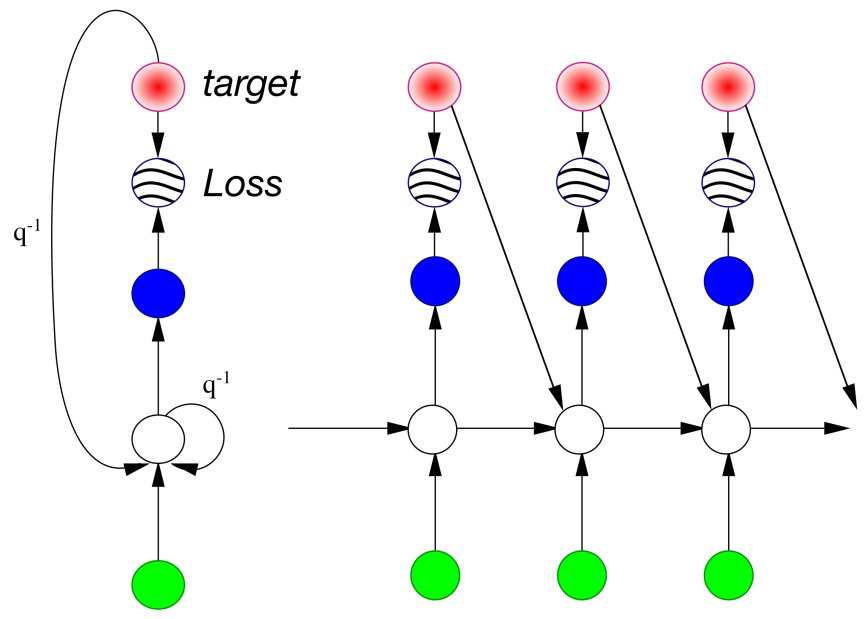
\includegraphics[width=8cm]{Images/teacher-forcing.jpg}
    \caption{Teacher Forcing in a RNN architecture}
    \label{fig:teacher-forcing}
\end{figure}

\noindent Using teacher forcing, the hidden state will be:

$$ h^{(t)} = \sigma \left( U x^{(t)} + W h^{(t-1)} + Z y^{(t - 1)} + b \right) $$

\newpage
\noindent In both feedback from the output and teacher forcing the $Z$ matrix represents a weight matrix that defines the connection between the previous output $o^{(t-1)}$ and the current hidden state $h^{(t)}$. Basically it controls how much influence the previous output has on the current hidden state. As every weight matrix, their values are learned during the training of the Recurrent Neural Network.


\subsection{Bidirectional Recurrent Neural Networks}

When the the sequence is not temporal (or we are processing the data off-line) we can use Bidirectional Recurrent Neural Networks. In this architecture, the output depends both on past and future values of the sequence.

\begin{figure}[h]
    \centering
    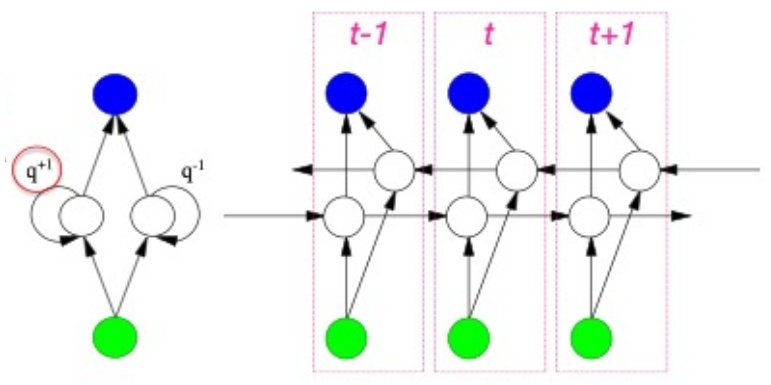
\includegraphics[width=9cm]{Images/bidirectional.jpg}
    \caption{Bidirectional Recurrent Neural Network}
    \label{fig:bidirectional}
\end{figure}

\noindent The output equation for a Bidirectional Recurrent Neural Network  will be:

$$ o^{(t)} = \sigma \left(V^{(p)} {h_p}^{(t)} + V^{(f)} {h_f}^{(t)} + c \right) $$

$$ h_p^{(t)} = \sigma \left( U^{(p)} x^{(t)} + W^{(p)} {h_p}^{(t-1)}  \right)  ~~~~~ h_f^{(t)} = \sigma \left( U^{(f)} x^{(t)} + W^{(f)} {h_f}^{(t+1)}  \right) $$

\noindent where $h_p^{(t)}$ encodes the hidden state for the past history and $h_f^{(t)}$ does the same for the future history.

\noindent All these architectural features (and others...) are orthogonal, meaning that they can be combined together.

\newpage
\section{Encoder-Decoder Sequence-to-Sequence Architectures}

Until now we have consider the Recurrent Neural Networks able to map an input sequence to a fixed-size vector, a fixed-size vector to a sequence and an input sequence to an output sequence of the same length. However, we haven't consider an architecture able to map an input sequence to an output sequence which is not necessarily of the same length. This comes up in many applications, such as speech recognition or machine translation.

The simplest Recurrent Neural Network architecture for mapping a variable-length sequence to another variable-length sequence is called the encoder-decoder or sequence-to-sequence architecture. The idea is very simple. First, an encoder processes an input sequence $X = x^{(1)}, ..., x^{(n_x)}$ and emits a context $C$ which represents a semantic summary of the input sequence. On the other hand, the decoder is conditioned on that fixed-length vector to generate the output sequence $Y = y^{(1)}, ..., y^{(n_y)}$.



\begin{figure}[h]
    \centering
    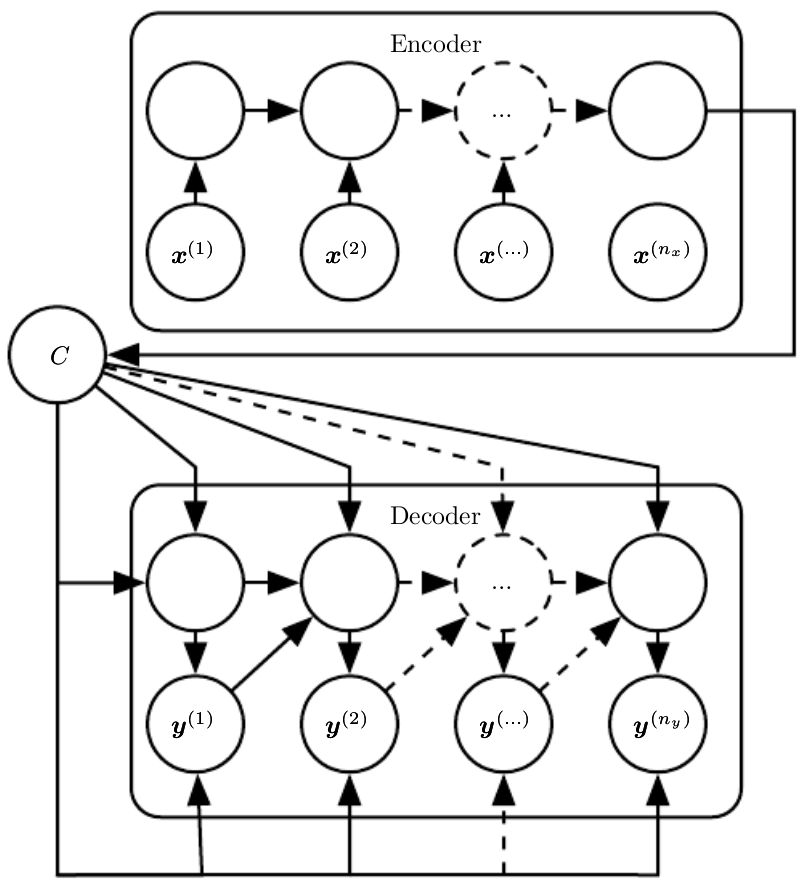
\includegraphics[width=10cm]{Images/encoder-decoder.png}
    \caption{Encoder-Decoder Architecture}
\end{figure}

\noindent In a sequence-to-sequence architecture, the two Recurrent Neural Networks are trained jointly to maximize the average of $\log P \left( y^{(1)}, ..., y^{(n_y)} | x^{(1)}, ..., x^{(n_x)}  \right) $ over all the pairs of $x$ and $y$ sequences in the training set. The last state $h^{(n_x)}$ of the encoder Recurrent Neural Network is typically used as a representation $C$ of the input sequence that is provided as input to the decoder Recurrent Neural Network.

\noindent One clear limitation of this architecture is when the context $C$ output by the encoder Recurrent Neural Network has a dimension that is too small to properly summarize a long sequence. To solve that, alternatives such as using an attention mechanism have found to be successful.

\newpage
\section{The Challenge of Long-Term Dependencies}

When trying to learn long-term dependencies in Recurrent Networks we face a major problem derived from how gradients propagated over many stages tend to either vanish or explode. Moreover, even by assuming that the parameters are stable, the difficulty with long-term dependencies arises from the exponentially smaller weights given to long-term interactions (involving the multiplication of many Jacobians) compared to short-term ones. 

\noindent We can look further by considering that the recurrence relation resembles a matrix multiplication.

$$h^{(t)} = W^{T} h^{(t-1)}$$

\noindent Iterating we get:

$$h^{(t)} = \left(W^{t} \right) ^T   h^{(0)}$$

\noindent If we consider that $W$ admits an eigendecomposition of the form

$$ W = Q \Lambda Q^T $$

\noindent with orthogonal $Q$, the recurrence may be simplified further to

$$ h^{(t)} = Q^T \Lambda^t Q h^{(0)} $$

\noindent The eigenvalues are raised to the power of $t$ causing eigenvalues with magnitude less than one to decay to zero and eigenvalues with magnitude greater than one to explode. Any component of $h^{(0)}$ that is not aligned with the largest eigenvector will eventually be discarded. This problem is particular to recurrent networks.

\noindent In practice, the experiments show that as we increase the span of the dependencies that need to be captured, gradient-based optimization becomes increasingly difficult, with the probability of successful training of a traditional Recurrent Neural Network via Stochastic Gradient Descent rapidly reaching 0 for sequences of only length 10 or 20.

\newpage
\section{Gated Recurrent Unit}

A Gated Recurrent Unit is a Neural Network architecture designed to address some of the limitations of traditional Recurrent Neural Networks. Same as Recurrent Neural Networks at each time step it receives as input the current state $x^{(t)}$ and the hidden state $h^{(t-1)}$ of the previous step and outputs the hidden state $h^{(t)}$ at the current time.

\begin{figure}[h]
    \centering
    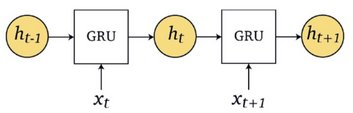
\includegraphics[width=8cm]{Images/gru-schema.jpg}
    \caption{GRU schema}
    \label{fig:gru-schema}
\end{figure}

\noindent The Gated Recurrent Unit addresses the vanishing/exploding gradient problem associated with traditional Recurrent Neural Networks by employing gating mechanisms that carefully control the flow of information through a combination of addition and multiplication operations. These mechanisms consist of the update  gate $z^{(t)}$, reset gate $r^{(t)}$, and the candidate hidden state $\hat{h}^{(t)}$.



\begin{figure}[h]
    \centering
    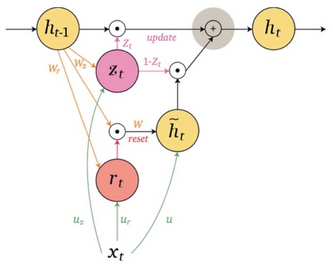
\includegraphics[width=8cm]{Images/gru-architecture.png}
    \caption{Gated Recurrent Unit Architecture}
    \label{fig:gru-architecture}
\end{figure}


\noindent Let's review these gates in more detail:


\subsection{Update Gate}

The update gate $z^{(t)}$ determines how much of the previous hidden state should be retained and is defined as a combination of the current state $x^{(t)}$ and the previous state $h^{(t-1)}$::

$$ z^{(t)} = \sigma \left( W_z h^{(t-1)} + U_z x^{(t)} \right)  $$

\begin{figure}[h]
    \centering
    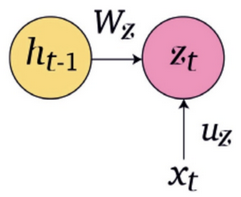
\includegraphics[width=3cm]{Images/update-gate.png}
    \caption{Update Gate}
    \label{fig:update-gate}
\end{figure}

\newpage
\noindent Because we are applying a sigmoid activation function, the output will be between 0 and 1. If the update gate is $z^{(t)} = 0$, then the current hidden state $h^{(t)}$ is the candidate hidden state $h^{(t)} = \hat{h}^{(t)}$. On the other hand, if the update gate is set to $z^{(t)} = 1$, then the output is the previous hidden state $ h^{(t)} = h^{(t-1)}$.

\begin{figure}[h]
\centering     %%% not \center
\subfigure[Update Gate $z^{(t)} = 0$]{\label{fig:update-gate-z0}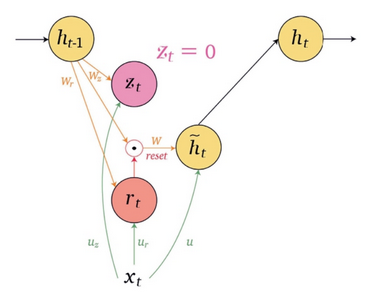
\includegraphics[width=6cm]{Images/update-gate-zt0.png}}
\subfigure[Update Gate $z^{(t)} = 1$]{\label{fig:update-gate-z1}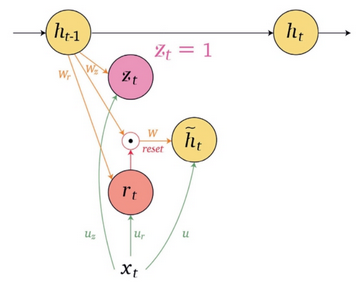
\includegraphics[width=6cm]{Images/update-gate-zt1.png}}
\label{fig:update-gate-zt}
\end{figure}


\noindent Considering that, the hidden state $h^{(t)}$ at time t is a linear interpolation between the previous hidden state $h^{(t-1)}$ and the current candidate $\hat{h}^{(t)}$, which is controlled by the update gate $z^{(t)}$

$$ h^{(t)} = z^{(t)} \odot h^{(t-1)} + (1 - z^{(t)}) \odot \hat{h}^{(t)} $$

\begin{figure}[h]
    \centering
    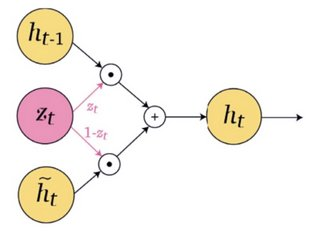
\includegraphics[width=5cm]{Images/gru-update-gate1.jpg}
    \caption{The Update Gate is Used for Interpolation}
    \label{fig:update-gate}
\end{figure}

\subsection{The Candidate}

The candidate hidden state $\hat{h}^{(t)}$ represents the proposed new hidden state that will be considered as an update to the current hidden state and is defined  as combination of the current state $x^{(t)}$ and the previous hidden state $h^{(t-1)}$ and modulated by the reset gate $r^{(t)}$. 

$$ \hat{h}^{(t)} = \phi ( W (r^{(t)} \odot h^{(t-1)}) + U x^{(t)} )  $$

The hyperbolic tangent function applied to the end result ensures that the candidate hidden state values are squashed between the -1 to 1 range, which helps maintain numerical stability in the model.

\begin{figure}[h]
    \centering
    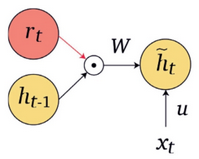
\includegraphics[width=3cm]{Images/candidate.png}
    \caption{Gated Recurrent Unit Candidate }
    \label{fig:candidate}
\end{figure}

\newpage
\subsection{Reset Gate}

The reset gate $r^{(t)}$ is responsible for determining how much of the previous hidden state $h^{(t-1)}$ should be reset or forgotten before computing the candidate hidden state $\hat{h}^{(t)}$.


$$ r^{(t)} = \sigma (W_r h^{(t-1)} + U_r x^{(t)}) $$

\noindent The reset gate is calculated using a sigmoid activation function, which produces values between 0 and 1, similar to the update gate.

\noindent If the reset gate is set to $r^{(t)} = 0$ then the candidate $\hat{h}^{(t)}$ is a function of the current state $x^{(t)}$ such that $\hat{h}^{(t)} = \phi \left( U x^{(t)} \right)$, forgetting the previous hidden state $h^{(t-1)}$. Instead if the reset gate is set to $r^{(t)} = 1$ then the candidate is also a function of the previous state $h^{(t-1)}$.

\begin{figure}[h]
\centering     %%% not \center
\subfigure[Reset Gate $r^{(t)} = 0$]{\label{fig:reset-gate-z0}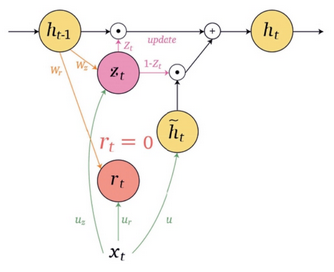
\includegraphics[width=5.5cm]{Images/reset-gate-rt0.png}}
\subfigure[Reset Gate $r^{(t)} = 1$]{\label{fig:reset-gate-z1}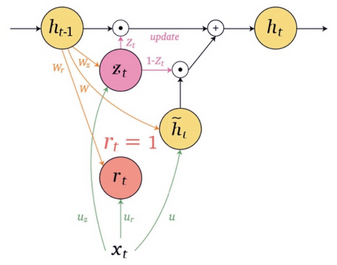
\includegraphics[width=5.5cm]{Images/reset-gate-rt1.png}}
\label{fig:reset-gate-rt}
\end{figure}

\noindent Together with the update gate and candidate hidden state, the reset gate plays a crucial role in determining how the GRU manages its memory and captures relevant information from the sequential data.

\subsection{Special Functionality}

\noindent If $z^{(t)} = 0$ and $r^{(t)} = 0$ then the hidden state is only dependent on the current state \linebreak $h^{(t)} = \phi \left( U x^{(t)} \right)$, forgetting the previous hidden state $h^{(t-1)}$.

\begin{figure}[h]
    \centering
    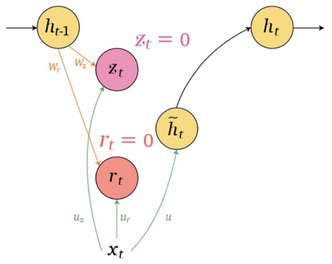
\includegraphics[width=5cm]{Images/GRUr0z0.png}
    \caption{Gated Recurrent Unit with $r^{(t)} = 0$ and $z^{(t)} = 0$}
    \label{fig:gru-r0-z0}
\end{figure}

\newpage
\noindent Instead if $z^{(t)} = 0$ and $r^{(t)} = 1$ the Gated Recurrent Unit is reduced to a vanilla Recurrent Neural Network such that $h^{(t)} = \hat{h}^{(t)} = \phi \left( W h^{(t-1)} + U x^{(t)} \right)$

\begin{figure}[h]
    \centering
    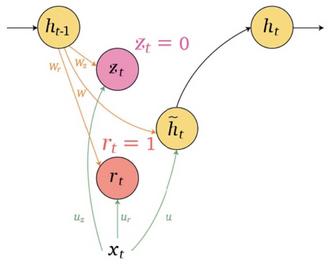
\includegraphics[width=5cm]{Images/GRUr1z0.png}
    \caption{Gated Recurrent Unit with $r^{(t)} = 1$ and $z^{(t)} = 0$}
    \label{fig:gru-r1-z0}
\end{figure}

\noindent Therefore, the careful management of information through these gates allows to avoid the vanishing gradient problem by learning when to update their memory and when to forget, making them more effective at capturing long-range dependencies in sequential data than vanilla Recurrent Neural Networks. 


\section{Long Short Term Memory (LSTM)}

Long Short-Term Memory is another specialized type of Recurrent Neural Network architecture specifically designed to address the vanishing/exploding gradient problem associated with Recurrent Neural Networks. They achieve this by incorporating gating mechanisms that control the flow of information. These gating mechanisms include the input gate $i^{(t)}$, the forget gate $f^{(t)}$, the output gate $o^{(t)}$ and the memory gate $c^{(t)}$. Additionally, a candidate memory $\hat{c}^{(t)}$ is also introduced.

\begin{figure}[h]
    \centering
    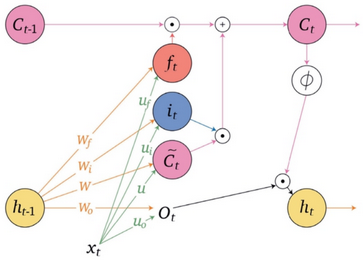
\includegraphics[width=7cm]{Images/lstm-architecture.png}
    \caption{Long Short Term Memory Architecture}
    \label{fig:lstm-architecture}
\end{figure}


\noindent At each time step, it receives as input the current state $x^{(t)}$, the hidden state $h^{(t-1)}$ and a memory cell $c^{(t-1)}$ of the previous time step, and outputs the hidden state $h^{(t)}$ and memory cell $c^{(t)}$ at time t. The memory cells propagate information from the previous state to the next, whereas the hidden states determine the way in which that information is propagated. 

\begin{figure}[h]
    \centering
    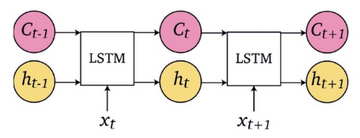
\includegraphics[width=6cm]{Images/lstm-sequential.png}
    \caption{Long Short Term Memory}
    \label{fig:lstm-seq}
\end{figure}

\subsection{The Forget Gate}

The forget gate $f^{(t)}$ is responsible for determining how much information from the previous cell state $c^{(t-1)}$ should be forgotten or retained when processing a new input at time step $t$ and is implemented as a combination of the current state $x^{(t)}$ and the previous state $h^{(t-1)}$:

$$ f^{(t)} = \sigma \left( W_f h^{(t-1)} + U_f x^{(t)}   \right) $$

\begin{figure}[h]
    \centering
    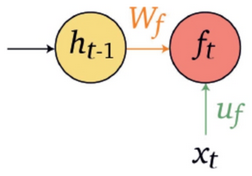
\includegraphics[width=3cm]{Images/lstm-forget-gate.png}
    \caption{Long Short Term Memory forget gate}
    \label{fig:lstm-forget-gate}
\end{figure}

\noindent The forget gate applies a sigmoid activation function to its output to produce values between 0 and 1, with 0 indicating complete forget of the previous memory cell $c^{(t-1)}$ and 1 indicating complete retention.



\begin{figure}[h]
    \centering
    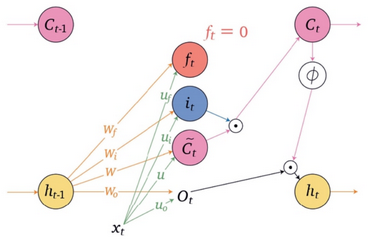
\includegraphics[width=8cm]{Images/lstm-forget-gate-f0.png}
    \caption{Long Short Term Memory forget gate for $f^{(t)} = 0$}
    \label{fig:lstm-forget-gate-f0}
\end{figure}

\subsection{Input Gate}

The input gate $i^{(t)}$ is responsible for determining how much new information should be added to the cell state $c^{(t)}$ at time step $t$ based on the current input $x^{(t)}$ and the previous hidden state $h^{(t-1)}$. 

$$ i^{(t)} = \sigma \left( W_i h^{(t-1)} + U_i x^{(t)} \right) $$

\begin{figure}[h]
    \centering
    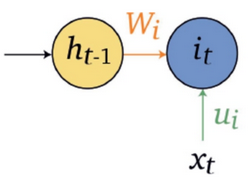
\includegraphics[width=3cm]{Images/lstm-input-gate.png}
    \caption{Long Short Term Memory input gate}
    \label{fig:lstm-input-gate}
\end{figure}

\newpage
\noindent The input gate is implemented using a sigmoid activation function to produce values between 0 and 1. Values close to 0 in the input gate prevent new information from being added, while values close to 1 allow new information to be fully integrated into the cell state. This mechanism enables to selectively update and maintain information in the internal memory, making them effective at capturing both short-term and long-term dependencies in sequential data.

\begin{figure}[h]
    \centering
    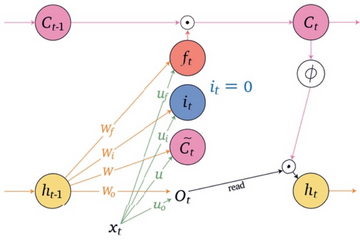
\includegraphics[width=8cm]{Images/lstm-input-gate-i0.png}
    \caption{Long Short Term Memory input gate for $i^{(t)} = 0$}
    \label{fig:lstm-input-gate-i0}
\end{figure}

\subsection{Memory Gate}

The memory cell state $c^{(t)}$ represents the internal memory of the LSTM and is designed to store and carry information over long sequences. It is updated at each time step based on the previous memory cell state $c^{(t-1)}$ and the candidate memory cell $\hat{c}^{(t)}$ at the current time step and controlled by both the input gate $i^{(t)}$ and forget gate $f^{(t)}$.

$$ c^{(t)} = f^{(t)} c^{(t-1)} + i^{(t)} \hat{c}^{(t)}$$

\begin{figure}[h]
    \centering
    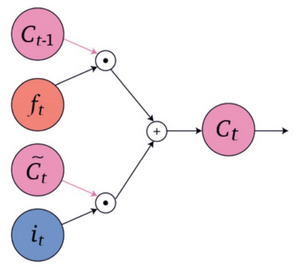
\includegraphics[width=4cm]{Images/lstm-memory-gate.png}
    \caption{Long Short Term Memory memory gate}
    \label{fig:lstm-memory-gate}
\end{figure}

\noindent Notice how if the forget gate $f^{(t)}$ is close to 0 the memory cell at time $t$ will ignore the information given by the previous time step. Meanwhile if the input gate $i^{(t)}$ is close to 0 the memory cell at time $t$ will ignore the information given by the new information from the candidate memory cell state. 

\newpage
\subsection{Candidate Memory}

The candidate memory cell state $\hat{c}^{(t)}$ represents the proposed new information that can be added to the memory cell state $c^{(t)}$ at the current time step $t$. It is computed based on the current input $x^{(t)}$ and the previous hidden state $h^{(t-1)}$.

$$ \hat{c}^{(t)} = \phi \left( W h^{(t-1)} + U x^{(t)} \right) $$

\begin{figure}[h]
    \centering
    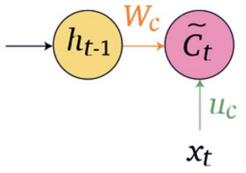
\includegraphics[width=3cm]{Images/lstm-candidate-memory.png}
    \caption{Long Short Term Memory Candidate Memory}
    \label{fig:lstm-candidate-memory}
\end{figure}

\noindent The hyperbolic tangent function ensures that the values are squashed to the range between -1 and 1, making the proposed information numerically stable. 

\subsection{Output Gate}

The output gate $o^{(t)}$ is responsible for determining how much of the updated memory cell state $c^{(t)}$ should be used to produce the output at the current time step. The output gate takes the current input $x^{(t)}$ and the previous hidden state $h^{(t-1)}$ as inputs and is implemented using a sigmoid activation function to produce values between 0 and 1. Values close to 0 in the output gate prevent information from the memory cell state from affecting the output, while values close to 1 allow the memory cell state to strongly influence the output.

$$ o^{(t)} = \sigma \left( W_o h^{(t-1)} + U_o x^{(t)}     \right)   $$

\begin{figure}[h]
    \centering
    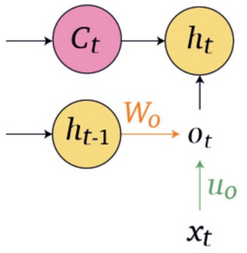
\includegraphics[width=3cm]{Images/lstm-output-gate.png}
    \caption{Long Short Term Memory output gate}
    \label{fig:lstm-output-gate}
\end{figure}

\noindent Where the hidden state $h^{(t)}$ represents the output of the LSTM at each time step. Basically, it represents the information that the LSTM has chosen to propagate to the next time step, considering both the memory cell state and the importance assigned to it by the output gate.

$$ h^{(t)} = o^{(t)} \phi \left( c^{(t)}  \right)$$

\subsection{Peephole Connections}

Peephole connections are a modification to the standard Long Short-Term Memory architecture. These connections allow the gates of the LSTM to have direct access to the previous cell state $c^{(t-1)}$ in addition to the current input $x^{(t)}$ and hidden state $x^{(t)}$. This additional information can improve the ability to control information flow. 

\newpage
\noindent The standard LSTM gates input gate $i^{(t)}$, forget gate $f^{(t)}$, and output gate $o^{(t)}$ are computed without considering the previous cell state. With peephole connections, these gates are modified to include direct access to $c^{(t-1)}$.

forget gate: $ f^{(t)} = \sigma \left( W_f h^{(t-1)} + P_f c^{(t-1)} + U_f x^{(t)} \right)$

input gate: $ i^{(t)} = \sigma \left( W_i h^{(t-1)} + P_i c^{(t-1)} + U_i x^{(t)} \right)$

output gate: $ o^{(t)} = \sigma \left( W_o h^{(t-1)} + P_o c^{(t-1)} + U_o x^{(t)} \right)$

\begin{figure}[h]
    \centering
    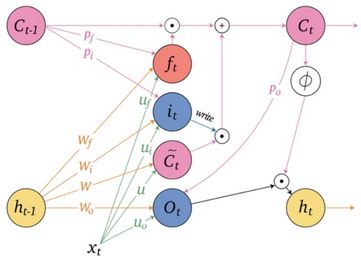
\includegraphics[width=6.5cm]{Images/lstm-peepholes.png}
    \caption{Long Short Term Memory with peepholes}
    \label{fig:lstm-peephole}
\end{figure}

\noindent Therefore, Long Short Term-Memory networks are effective in mitigating the vanishing and exploding gradient problems by incorporating gating mechanisms, careful activation functions, and controlled information flow. These mechanisms allow to learn and capture long-range dependencies in sequential data and enable the training of deep networks with more stability and better gradient flow. 


\subsection{Gated Recurrent Unit vs Long Short Term Memory}

\noindent Comparing the interpolation of the new candidate in the Gated Recurrent Unit with the interpolation of the new memory cell in the Long Short Term Memory shows that the update gate $z^{(t)}$ controls the amount of the new candidate to pass in the Gated Recurrent Unit, whereas the input gate controls the amount of the new candidate memory to pass in the Long Short Term Memory. Interpolation in the Gated Recurrent Unit is controlled by a single parameter $z^{(t)}$, whereas in the LSTM interpolation is controlled by two separate parameters $i^{(t)}$ and $f^{(t)}$.

\begin{figure}[h]
\centering     %%% not \center
\subfigure[Gated Recurrent Unit candidate interpolation]{\label{fig:gru-candidate-interpolation}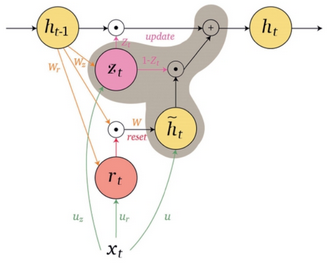
\includegraphics[width=7cm]{Images/gru-candidate-interpolation.png}}
\subfigure[Long Short Term Memory candidate interpolation]{\label{fig:lstm-candidate-interpolation}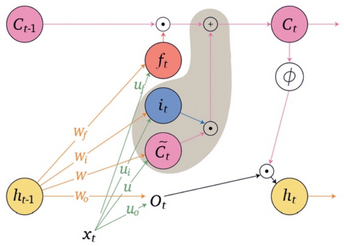
\includegraphics[width=7cm]{Images/lstm-candidate-interpolation.png}}
\label{fig:lstm-gru-interpolation}
\end{figure}

\newpage
\noindent Comparing the Gated Recurrent Unit reset gate controlling the candidate hidden state with the Long Short Term Memory input gate controlling the candidate memory cell shows the modulation of the candidate in both units.

\begin{figure}[h]
\centering     %%% not \center
\subfigure[Gated Recurrent Unit candidate]{\label{fig:gru-candidate-interpolation}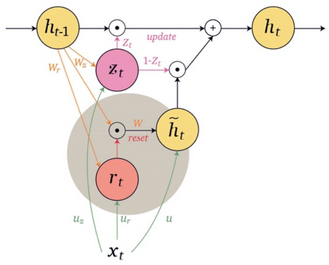
\includegraphics[width=7cm]{Images/gru-candidate.png}}
\subfigure[Long Short Term Memory candidate]{\label{fig:lstm-candidate-interpolation}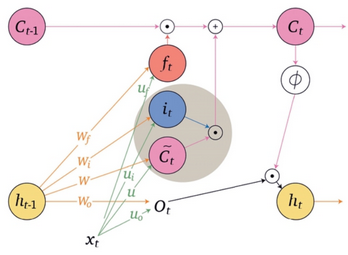
\includegraphics[width=7cm]{Images/lstm-candidate.png}}
\label{fig:lstm-gru-candidate}
\end{figure}

\noindent Both GRUs and LSTMs address the vanishing gradient problem and excel in sequential data tasks, LSTMs offer more advanced memory management and fine-grained control over information flow. The choice between the two depends on the specific requirements of the task, available data, and computational resources. GRUs are a more lightweight option for many applications, while LSTMs are often preferred when complex, long-range dependencies need to be modeled.


\section{Reservoir Computing Networks}

Reservoir Computing Networks offer an alternative architectural approach to mitigate the vanishing or exploding gradient problem commonly encountered in Recurrent Neural Networks. In a standard RNN, the recurrent weights linking the previous hidden state $h^{(t-1)}$ to the current state $h^{(t)}$, as well as the input weights connecting the input $x^{(t)}$ to $h^{(t)}$, can be challenging to learn effectively. Reservoir Computing Networks address this by introducing a reservoir of $N$ units with fixed, randomly initialized connections. The weight matrices governing connections between these hidden units, as well as those between the hidden units and the input, remain unaltered. This design choice is made to ensure that the recurrent hidden units are able to capture the temporal dependencies of past inputs, while only the output weights are subject to learning.

\begin{figure}[h!]
    \centering
    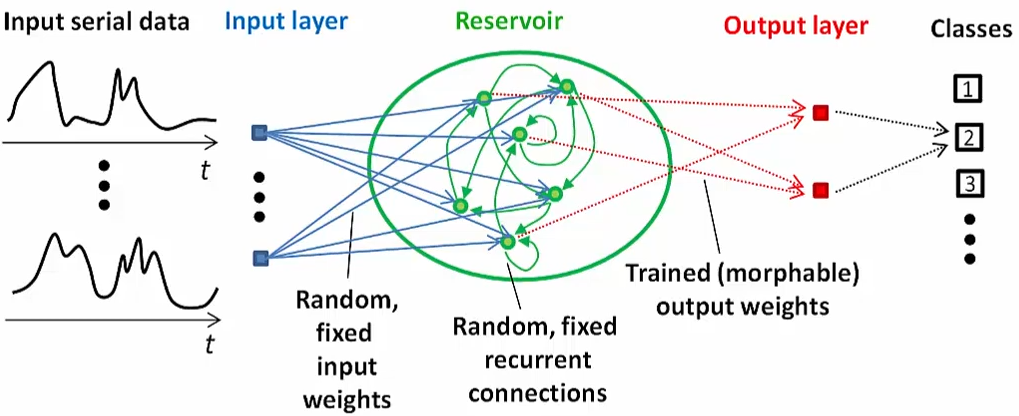
\includegraphics[width=10cm]{Images/reservoir-network.png}
    \caption{Reservoir Network}
\end{figure}


\noindent The distinctive feature of Reservoir Computing Networks lies in their introduction of a reservoir, a dynamic layer composed of $N$ internal units. This reservoir is characterized by fixed, randomly initialized connections, both within the reservoir and between the reservoir and the input layer. These fixed connections create a dynamic system with a rich state space, allowing the reservoir to naturally capture and propagate information from past inputs to the present state. This is achieved by leveraging the Echo State Property, which encourages the reservoir's internal dynamics to quickly forget initial conditions and be primarily influenced by current inputs. 

\noindent In order to implement the reservoir computing network we need to have an internal memory for the internal units. In Echo State Machines the idea is to have as internal units standard recurrent neurons plus some units working as leaky integrators. This ones are defined by the following formula:

$$ h^{(t)} = (1 - a)h^{(t-1)} + \sigma \left( U x^{(t)} + W h^{(t-1)} \right) $$

where $a$ is the decay rate and is used to control how much of the memory from the previous time step is take into account. This is used in order to be able to keep long term dependencies. For $a=1$ this gives us the equation of the standard recurrent unit. Adding leaky integrators makes the reservoir to remember information from the past. In these type of reservoir network, reservoir's state echoes relevant information from the past inputs, contributing to its ability to capture temporal dependencies. 


\noindent In order to produce a rich set of dynamics, the reservoir should:
\begin{itemize}
    \item Be big. From hundreds to thousands of units.
    \item Be sparse and randomly connected. The number of connections should be low compared to the number of possible connections and those connections should follow a uniform distribution. Keep in mind that the input and output matrices should be dense in order to not lose information from the input or to the output.
    \item Satisfy the echo state property. The effect of the current state $h^{(t)}$ and the current input $x^{(t)}$ on a future state $h^{(t + \tau)}$ should vanish gradually as time passes $\tau \rightarrow \inf$. This basically means that the spectral-radius is $\rho(W) < 1$. The spectral-radius of a matrix is the maximum eigenvalue. This is done so the memory does not saturate. Even if the architecture is designed to learn long term dependencies there should be a way to forget part of them as the iterations go by.
\end{itemize}

\noindent Finally, in Reservoir Computing Networks, the learning process is focused on adapting the weights connecting the reservoir to the output layer. Only these output weights are subject to learning. Indeed the output is computed then as a simple linear combination of the input-excited reservoir which makes it a fast training. By confining the learning process to the output layer, the complexity of training is significantly reduced compared to traditional Recurrent Neural Networks.















